\section{Interessentanalyse}
I dette afsnit indflydelses- og medvirken matrixen blive anvendt, for at undersøge og prioritere interessenter for dette projekt. Dette undersøges for, at finde ressourcepersoner som gruppen kan gøre brug af gennem interviews. Disse personer vil være respondentgruppen til undersøgelse af den initierende problemstilling.
Jens Børsting nævnte i interviewet, at o-løbere er interessenter, da de ønsker en IT-løsning til sammenligning af løb, samt o-løbs trænere er interessenter, da de ønsker bedre træning, samt nedsat arbejdsbyrde.

Gruppen vil i dette afsnit undersøge diverse personer/grupper, der kan fungere som interessenter i projektet, altså en person der vil have nytte af eller kan bidrage til projektet.

\subsection{Aktører}
I dette projekt har gruppen fundet tre aktører med hjælp fra Jens Børsting, som gruppen mener er relevante til projektet. De forskellige aktører er henholdsvis o-løberne, trænerne og sportens forbund og foreninger. 

\subsubsection{O-løbere}
For at den enkelte o-løber skal kunne forbedre sig, er det vigtig at kunne sammenligne løberens rute detaljeret med andre. Lige nu er tiderne mellem hver post (stræktiderne) det eneste der kan sammenlignes og analyseres på. Her er det interessant for løberen at kigge på vejvalg og hastighed mellem posterne, og endda helt ned til de forskellige faser af delstrækkene. Til dette mangler der mere detaljeret data om løbet. Problemet håndteres i dag ved at sammenligne skemaer med stræktider og hvis muligt manuelt indtegne vejvalg på kortet efter løberens hukommelse. Derfor har den enkelte o-løber interesse i dette projekt, da der arbejdes med afvikling og opfølgning af træningen. 

\subsubsection{Træneren}
Træneren har interesse i at gøre de enkelte løbere bedre, træneren har derfor også interesse i at mindske arbejdet på planlægning og forberedelse af træningen, da der bruges meget tid med dette. Samtidigt vil træneren gerne kunne analysere den enkelte løbers tur detaljeret, ved at sammenligne løberens rute med andre løberes rute. Hvis løberen ikke kan huske hvor vedkommende har løbet, eller var faret vild, har træneren svært ved at give sikker og brugbar kritik, da det ikke kan ses på tiderne, præcis hvor den enkelte løber har været. Trænere har derfor interesse i et værktøj som kan hjælpe med planlægning og afviklingen af træningen, samt evaluering af den enkelte løbers tur.

\subsubsection{Forbund og foreninger}
O-løbernes forbund hedder Dansk Orienterings Forbund, også kaldt for DOF, som ligger under Dansk Idrætsforbund, DIF. Der er i alt 76 foreninger i DOF, med lidt under 7.000 medlemmer\citep{DIF}. DOF er med til at drive landsholdet, samt står for talentudviklingen inden for orienteringsløb. Dette gør DOF og foreningerne til interessenter i dette projekt, da de bl.a. ønsker deres løbere skal blive så gode som mulige. Derudover kunne de have nogle krav til en evt. løsning. \citep{DIF}

\subsubsection{Frivillige}
I interviewet med Claus Bobach nævnte han, at det var frivillige der satte posterne ud for ham. Derudover er mange af de frivillige engageret i o-løb, da de er villige til at lave et strykke ubetalt arbejde, for at holde gang i klubben. Eksempelvis i Claus' klub, har de nogle der sørger for mad og drikke efter træninger, samt før nævnt hjælper til med posterne.


\subsection{Prioriteringen}
Ved prioritering af interessenter, bliver indflydelse- og medvirken matrixen anvendt. Denne matrice deles op i fire rum, hvor hvert rum er scaleret efter ”indflydelse på projektet” og ”afgørende medvirken i projektet”. Dette giver rum for diskussion af de enkelte interessenter, for at undersøge hvilke interessenter, der skal tages kontakt til, for at få svar på den initierende problemstilling.
Gruppen har i denne rapport meget få interessenter, hvilket medfører, at de enkelte interessenter hurtigt bliver ressourcepersoner.

\textbf{Eksterne interessenter} har hverken en stor indflydelse eller en stor medvirken i projektet. Det betyder at der ikke nødvendigvis skal tages stor hensyn til denne gruppe af interessenter.\newline 
\textbf{Den grå eminence} har stor mulighed for at påvirke beslutninger i projektet, men deres medvirken er ikke særlig stor i projektet, dette vil ofte være en person med en magtfuld stilling eller ledelses position. \newline
\textbf{Gidsler} har ikke stor mulighed for at træffe beslutninger i projektet, men deres aktive medvirken er vigtig for projektet.\newline
\textbf{Resourcepersoner} har både stor indflydelse og stor medvirken, da det er denne gruppe der skal inddrages i projektet. Denne gruppe har både erfaring eller faglige kompetencer indenfor området. \newline
  
O-løbere er i dette projektet sat som ressourceperson, da de kan give råd og vejledning til, hvordan deres træning og løb fungere, samt undersøge om der er ting der kan forbedre o-løbernes løb. Dette gælder både inden løb og efter løbet.

Trænere er sat som ressourceperson for projektet, da de ligesom o-løberne har et stort indblik i hvordan orienteringsløb fungere, og hvordan det måske kan optimeres eller forbedres. 

DOF og foreningerne er i dette projekt grå eminence, da de kan have en indflydelse på projektet. Herudover kan de have nogle krav og regler til en løsning. Deres medvirken er dog ikke nødvendig for at projektet skal kunne blive en succes.

I dette projekt har gruppen valgt at placere de frivillige som gidsler. Da de frivillige ikke har nogen indflydelse på hvordan projektet bliver lavet, men de laveer stadig et stykke arbejde som er værd at tænke over i løsningen.    

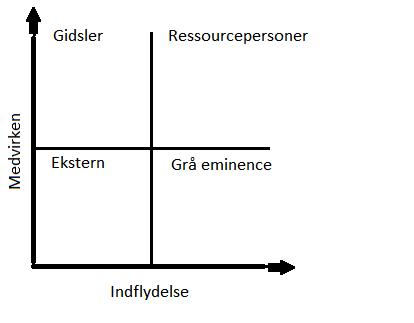
\includegraphics[width=0.70\textwidth]{billeder/matrix}
\vspace{0.20cm}

\subsubsection{Opsummering}
Ud fra interessentanalysen, er gruppen kommet frem til at o-løberne og trænerne, er de vigtigste interessenter, og er derfor også blevet sat som ressourcepersoner i dette projekt. Derfor har gruppen valgt at kontakte de to grupper af interessenter, og gennemføre et interview med dem. 
